\chapter{Models}


\section{Colorful Image Colorization}
\label{sec:colorful}

The first approach to colorization discussed in this thesis is will be using
the architecture described by Zhang et al. in their paper \textit{Colorful Image Colorization} 
\citep{zhang2016colorful}. Their architecture was specifically created to 
address the inherent problem of multimodality described in section \ref{sec:multimodality}.

\subsection{Architecture}

The architecture of this model was specifically built to address the problem
of multimodality we encounter when colorizing. The authors tackled that problem 
by rephrasing the task of colorization as a classification problem, where the 
usual approach was to treat it as a regression problem.

\begin{figure}[!ht]
	\centering
	\begin{subfigure}{.24\textwidth}
		\centering
		\includegraphics[width=\linewidth]{plot/lab_bins/20}
	\end{subfigure}
	\begin{subfigure}{.24\textwidth}
		\centering
		\includegraphics[width=\linewidth]{plot/lab_bins/40}
	\end{subfigure}
	\begin{subfigure}{.24\textwidth}
		\centering
		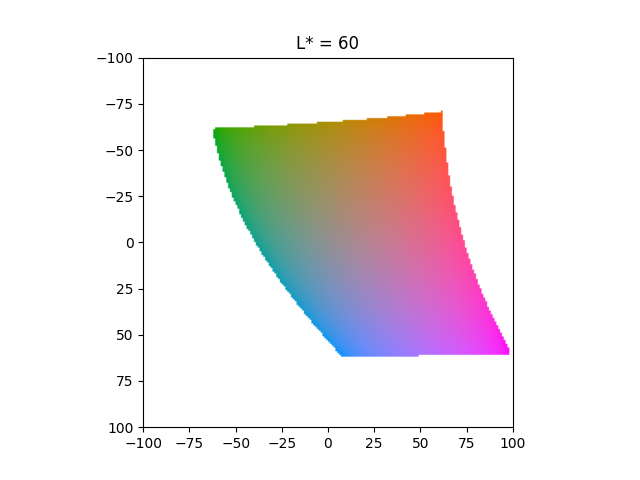
\includegraphics[width=\linewidth]{plot/lab_bins/60}
	\end{subfigure}
	\begin{subfigure}{.24\textwidth}
		\centering
		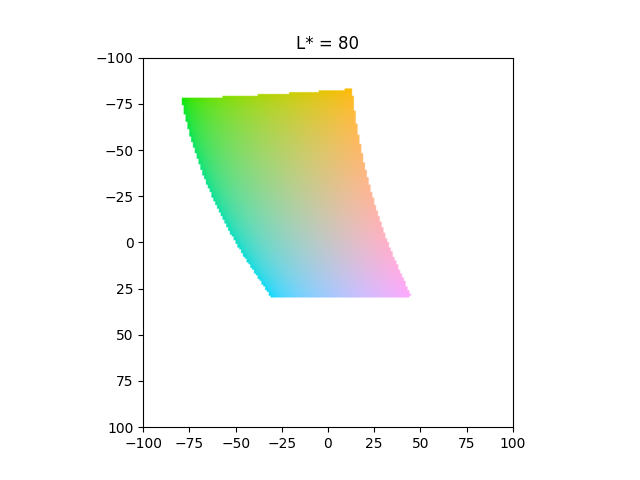
\includegraphics[width=\linewidth]{plot/lab_bins/80}
	\end{subfigure}
    \caption{Quantized \textbf{a*b*} bins for different \textbf{L*} values}
	\label{fig:lab_bins}
\end{figure}

Instead of predicting the exact \textbf{a*} and \textbf{b*} channel values 
for each pixel, this model outputs a probability distribution over 313 seperate classes. 
Each class represents one quantized \textbf{a*b*} bin. 
The $Q$-bins, each $10\times10$ in size, cover the whole \textbf{a*b*} gamut as seen
in figure \ref{fig:lab_bins}.

\begin{figure}[!ht]
	\centering
	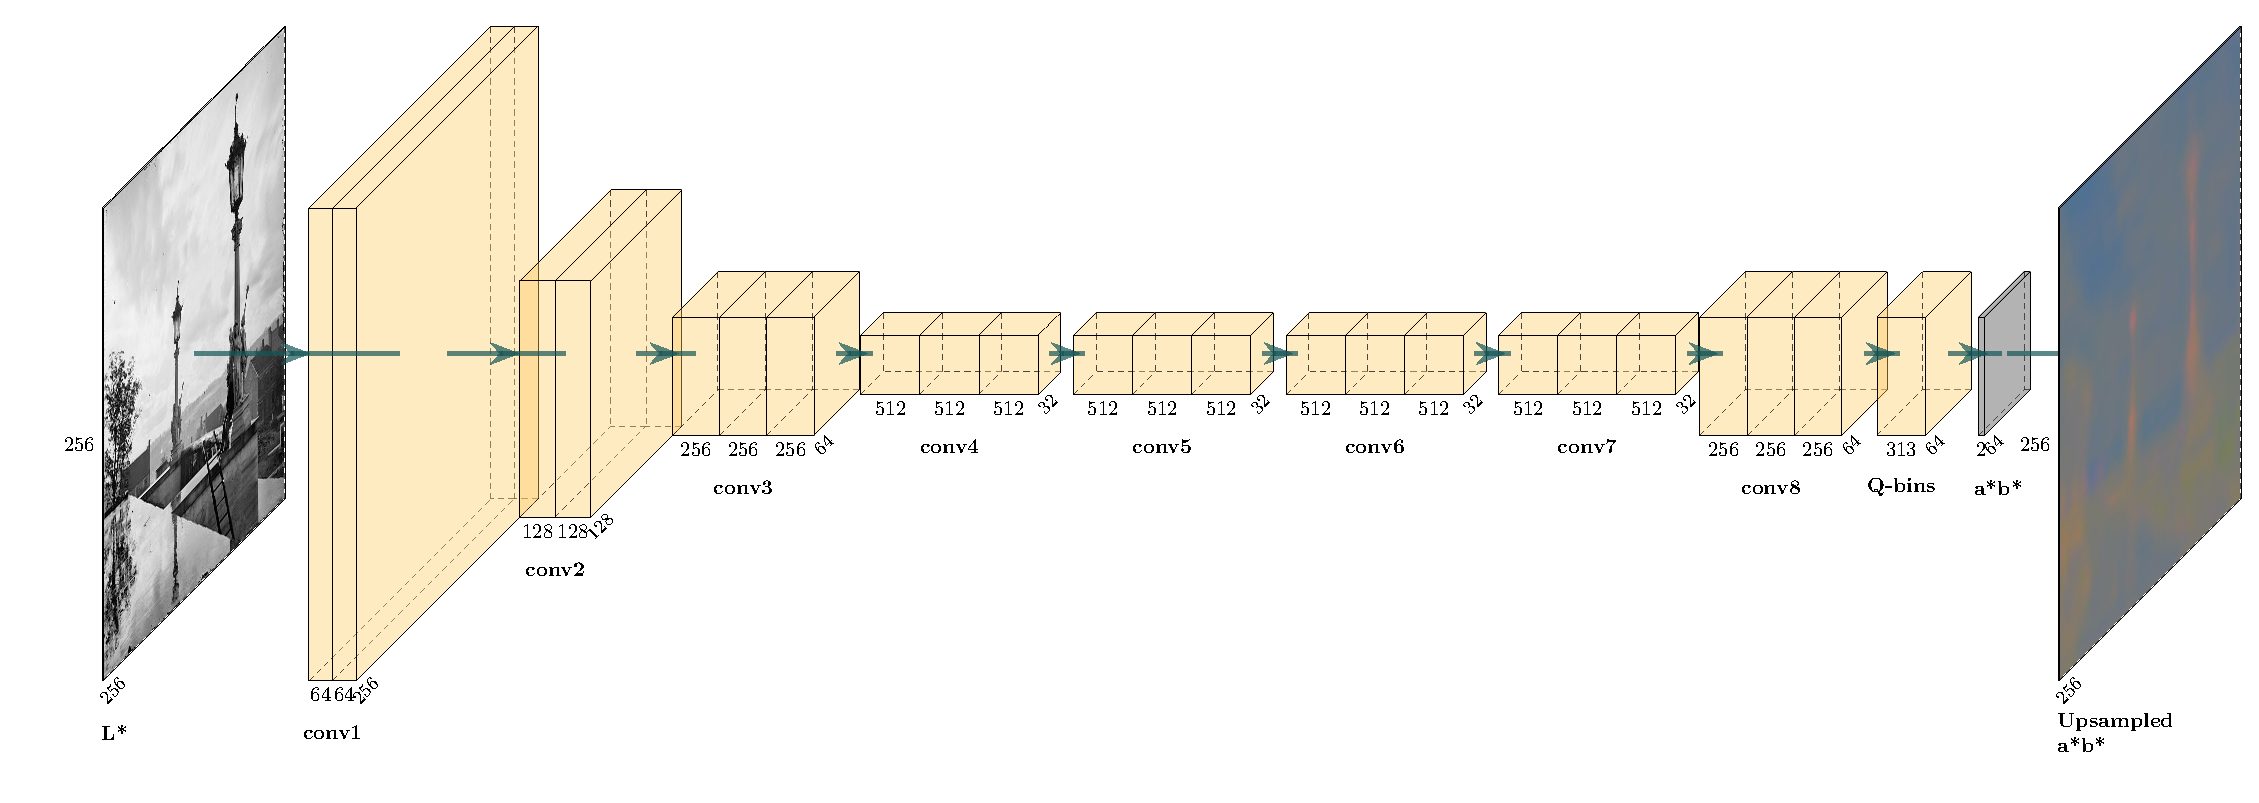
\includegraphics[width=\linewidth]{architecture/colorful}
    \caption{The architecture of the \textit{Colorful Image Colorization} model. 
	The eight convolutional blocks and the layer mapping the output to the probability 
	distribution over the $Q$-bins are colored in yellow, and probability to \textbf{a*b*}
	mapping in black}
	\label{fig:architecture_colorful}
\end{figure}

The model used is a modified version of the VGG \citep{simonyan2015vgg} network 
that was specifically created for classification. The model consists of eight
convolutional blocks and a convolutional-softmax pair for mapping the output to a
probability distribution over the 313 $Q$-bins.	All the convolutional blocks
consist of two to three convolutional-ReLU pairs (convolutional layer
paired with a ReLU activation \citep{abien2018relu}) and a batch normalization layer 
\citep{ioffe2015batchnorm} for normalizing the output of the block. 
The convolutional layers are all padded and have a kernel of size $3\times3$. There are 
no pooling layers in the network, the downsampling in the first three convolutional blocks 
is done by setting the stride in the last convolutional layer to $2$ instead.
To further increase the receptive field of each output distribution, à trous convolution
\citep{yu2016atrous} is used in the fifth and sixth layer, with the dilation set to $2$. 
Looking at the architecture of the network in figure \ref{fig:architecture_colorful},
we can see that the features are getting upsampled in the eighth block. The upsampling
is done by replacing the first layer of the block with a transposed convolution layer.
After the eighth block, a final convolution paired with softmax is applied to the 
features to get the probability distribution over the $Q$-bins. 

\subsection{Annealed mean}

To obtain the value of the \textbf{a*} and \textbf{b*} channels we could 
simply select the most likely color suggested by the colorizer On 
the other hand, we could calculate the weighted average over all the classes.
Somewhere in the middle of the two approaches lies the method proposed by 
the authors, they suggest a softmax-like calculation they named the annealed mean.
Using the annealed mean allows us to regulate how much we want to emphasize the 
most likely colors, or how close we want the result to be to the weighted 
average of the distribution.

Using the formula:

\begin{equation}
    W_T(p) = \frac{exp(log(p)/T)}{\sum_{q}{exp(log(p_q)/T)}}\label{eq:annealed_mean}
\end{equation}

we calculate the adjusted weights, where $p$ is the associated 
probability of a bin being the proposed color. $T$, which stands 
for temperature, is a hyperparameter of the function and it is used to 
adjust how drastically we want the colorization to be. When $T$ is set $1$
the weight is not adjusted and is equal to the probability $p$. On
the other hand, $T=0$ is an edge case where only the most probable bin 
gets assigned the weight of $1$. Programmatically that represents a problem 
as division  by zero results in an error, hence we implement a special case
for that situation where we map the probability distribution $\mathbf{p}$
to a one-hot encoded vector, with $1$ assigned to the $argmax(\mathbf{p})$
class.

As the sum over all the adjusted weights is $1$, the final color $\mathbf{c}$ 
for the pixel, given the probability distribution $\mathbf{p}$ is calculated 
using the formula:

\begin{equation}
    \mathbf{c} = \sum_{q}W_T(p_q) * \mathbf{c_q}\label{eq:weighed sum}
\end{equation}

\begin{figure}[!ht]
	\centering
	\begin{subfigure}{.19\textwidth}
		\centering
		\includegraphics[width=\linewidth]{img/colorful/temperature/100}
		\caption{$T=100$}
	\end{subfigure}
	\begin{subfigure}{.19\textwidth}
		\centering
		\includegraphics[width=\linewidth]{img/colorful/temperature/70}
		\caption{$T=70$}
	\end{subfigure}
	\begin{subfigure}{.19\textwidth}
		\centering
		\includegraphics[width=\linewidth]{img/colorful/temperature/40}
		\caption{$T=40$}
	\end{subfigure}
	\begin{subfigure}{.19\textwidth}
		\centering
		\includegraphics[width=\linewidth]{img/colorful/temperature/20}
		\caption{$T=20$}
	\end{subfigure}
	\begin{subfigure}{.19\textwidth}
		\centering
		\includegraphics[width=\linewidth]{img/colorful/temperature/0}
		\caption{$T=0$}
	\end{subfigure}
	\caption{Colorization of an image using different values of $T$}
	\label{fig:temperature}
\end{figure}

The effect that different values of $T$ have on the result of the colorization
can be seen in figure \ref{fig:temperature}. In the paper, the authors mention
that they got the best results using $T=0.38$. While that value might be the best
in general for fully automated colorization, individual photographs might benefit
from fine-tuning the hyperparameter. Higher temperature values usually result in 
lower overall saturation, while lower values yield crispier, but also more error-prone, results.

\begin{figure}[!ht]
	\centering
	\begin{subfigure}{.49\textwidth}
		\centering
		\includegraphics[width=\linewidth]{img/lab_channels/nature}
	\end{subfigure}
	\begin{subfigure}{.49\textwidth}
		\centering
		\includegraphics[width=\linewidth]{img/lab_channels/nature_4}
	\end{subfigure}
    \caption{Original image on the left, and the same image where the resolution of the \textbf{a*} and \textbf{b*} channels was reduced by a factor of four on the right}
	\label{fig:color4}
\end{figure}

In the end, the size of the output is 4 times smaller than the size of the input. 
Because of that, we upscale the output by a factor of 4 in the final step. That might
seem like a problem at first, but looking at figure \ref{fig:color4} we can see
that the \textbf{L*} channel is responsible for conveying most of the information, and
that the lower resolution of the \textbf{a*} and \textbf{b*} channels does not impact
the quality too much.

\subsection{Training}

The network was trained on the ImageNet dataset that, when filtered, contains
1.1 million photographs of different shapes and sizes. Before training, we first
have to do a little preprocessing to make the process of training easier. It is 
preferable that all the inputs are of the same size, as training batches on 
different-sized images cannot be done efficiently, hence all the images were 
converted to a uniform size. 

\begin{figure}[!ht]
	\centering
	\includegraphics[width=0.8\linewidth]{img/colorful/bitmap.png}
    \caption{
	The image is first resized to a size where the shorter of the two sides
	is $256$ pixels in length, afterwards a $256\times256$ square is 
	randomly cropped out of the resized image}
	\label{fig:crop}
\end{figure}

The only is the restriction for the input size is that both the width and height
of the input image should be a multiple $8$ for the model to work. That restriction
is present because of the downsampling in the first three convolutional blocks of
the network. When selecting the input size, we need to take into account that the
model has to have a good enough resolution to detect which objects are present. On 
the other hand, the resolution of the images should not be too high as that slows 
down the training process. The size of $256\times256$ is a good compromise between
the two conditions, as the network will have more than enough information to colorize, 
but also the process of training will not take an eternity. The process of resizing 
can be seen in figure \ref{fig:crop}.

The model was trained for 600 thousand iterations using the Adam optimizer \citep{diederik2015adam}
with a batch size of 40. The initial learning rate was $3\times10^-4$, and it was
reduced by a factor of $\sim$3 ($3\times10^{-4}$, $1\times10^{-4}$, $3\times10^{-5}$,
..., $1\times10^{-6}$) every 100 thousand iterations, or roughly every 4 epochs. 
Throughout the training, the optimizer parameters were static with the weight decay
being set to $1\times10^{-3}$ and $\beta_1$, $\beta_2$ having the value of $(0.9, 0.99)$.

\begin{algorithm}[!ht]
	\caption{Training step for the \textit{Colorful Image Colorization} model}
	\label{alg:colorful}
	\begin{algorithmic}		
		\Function {step}{$batch$, $network$, $optimizer$}		
			\State $l \leftarrow batch[:1]$	
			\State $ab \leftarrow batch[1:]$
			\State $predicted \leftarrow network.forward(l)$	
			\State $q\_bins \leftarrow encode(ab)$
			\State $loss \leftarrow CELoss(predicted, q\_bins)$
			\State $loss.backward()$
			\State $optimizer.step()$
		\EndFunction
	\end{algorithmic}
\end{algorithm}

One training step of the colorizer is outlined in figure \ref{alg:colorful}. 
Firstly we separate the \textbf{L*} from the \textbf{a*b*} channels, as \textbf{L*}
is the input, and \textbf{a*} and \textbf{b*} are wanted outputs. Next, 
we carry out a forward pass through the network and get the proposed color 
distribution for the images. At this point, we cannot calculate the loss of the
colorization as the \textbf{a*} and \textbf{b*} have to be encoded into 313 bins.
After the encoding we calculate the cross-entropy, calculate the gradients, and 
update the model.

\begin{figure}[!ht]
	\centering
	\includegraphics[width=0.5\linewidth]{img/colorful/distribution}
    \caption{Graph borrowed from the original paper \citep{zhang2016colorful}, 
	showing the overall distribution of color channel values in the ImageNet
	dataset, using a logarithmic scale (red indicates high, and blue low occurance)}
	\label{fig:distribution}
\end{figure}

The encoding of \textbf{a*} and \textbf{b*} could be done by finding the 
closest $Q$-bin and creating a one-hot vector representing that color. The 
problem with that representation is that we cannot express if the color
was somewhere in between of two bins. That's why the authors of the 
paper proposed encoding the color by applying a Gaussian kernel. That way
the closer the color is to the center of the bin the higher the associated
value of the class is. Another useful property of this encoding is that this way
the network can learn which bins are neighboring, as the encoder will only 
activate neighboring classes at the same time.

Unfortunately, the cross-entropy loss is usually implemented using labels as targets,
and not encoded vectors. While that approach is quite optimized and much faster, 
it does not suit our needs as we are soft-encoding the colors. That's why for 
the purpose of training this model we have to implement a custom multinomial 
cross-entropy loss.

Looking at figure \ref{fig:distribution} we can see that the colors are not 
equally distributed over the \textbf{L*a*b*} color space, on the contrary
the neutral colors (the ones closer to the center of the graph) are represented
at a much higher rate than marginal colors. To counter that disparity we can
rebalance the classes \citep{tantithamthavorn2020rebalancing}, giving the 
underrepresented classes an equal chance to get selected.

\subsection{Results}

\clearpage
\section{Generative Adversarial Networks for Colorization}
\label{sec:gan}

The second approach to colorization analyzed in this thesis comes in the form
of a generative adversarial network (abbr. \textit{GAN}) \citep{goodfellow2014generative}.
The main motivation for using GANs in this scenario is beacause of the 
generator-discriminator schema which has proven its usefulness in generating 
convincing data. No specific paper was used as a reference while implementing 
this model, but the papers by Nazeri et al. \citep{nazeri2018gan} and Isola 
et al. \citep{isola2017pix2pix} strongly influenced the design and training choices.

\subsection{Architecture}

The architecture of this model was ispired by the \textit{pix2pix} model proposed
by Isola et al. in 2017 for image-to-image translation tasks. Image colorization
was mentioned as one of many potential use cases for their model.

\subsubsection{Generative adversarial networks}

Generative adversarial networks are based on the idea of a \textit{game} between
two artificial neural networks. The first of the two networks, called the generator, 
has the task of generating plausible looking data. The second network, called the
discriminator, has to discern if the data it got was artificially generated by the
generator, or if it is genuine data.

\begin{figure}[!ht]
	\centering
	\includegraphics[width=0.7\linewidth]{img/gan/museum}
    \caption{Analogy for the way GANs work}
	\label{fig:museum}
\end{figure}

The tasks of the two networks can be concieved of as a rivarly between a forger
and a museum examiner outlined in figure \ref{fig:museum}.
The idea of generative adversarial networks is based on 


\subsubsection{Conditional GAN}

- Training is not only done on an adversarial basis, but the generator is also nudged in the right direction by another condition
- Ekstenzija formule za gresku gana

\subsubsection{Generator}

- U net Architecture
- Diagram of the network
- Numer of layers
- 

\subsubsection{Discriminator}

- Diagram
- Patch gan
- DCNN

\subsection{Training}

- algpseudocode (train discriminator/ train generator)
- Loss function proposed NIPS \citep{goodfellow2017nips}
- Problem with helvetica scenario \citep{goodfellow2014generative}
- Hard to validate the how it is going, only the conditional loss gives some insight, generally good if the fitness of the discriminator is up and down, which means that the generator and discriminator are fighting

\subsection{Results}

\section{Interactive Deep Colorization}
\label{sec:ideep}

- By the same autors as the first model
- One of 2 models proposed, global hints
- Nadogradnja prvog modela
Not fully automated
- Idea to give the operator a chance to influence the colorization of the image

\subsection{Architecture}
- the first model converted to u net
- As can be seen from the diagram the first 8 layers are the same
- additional 2 expansive layers + skip connections and skip convolutions

\subsection{Transfer learning}

- What is transfer learning:
	Dogradivanje
	- Training one model and applying the learned knowledge on another model
	
- The weights of the trained first model, in the end crucial as the model could not colorize without the initial push

\subsection{Global hints}


\subsection{Training}

\subsection{Results}